\documentclass[12pt]{article}
\usepackage[utf8]{inputenc}
\usepackage[T1]{fontenc}
\usepackage[french]{babel}
\usepackage{fullpage}
\usepackage{color}
\usepackage[table]{xcolor}
\usepackage{listings}
\usepackage{url}
\usepackage{graphicx}
\usepackage{caption}
\usepackage{tabto}
\usepackage{enumitem}
\usepackage{babel}
\usepackage{hyperref}
\hypersetup{colorlinks=false}
\usepackage{spverbatim}
\usepackage{dirtree}

\definecolor{darkWhite}{rgb}{0.94,0.94,0.94}

\lstset{
  aboveskip=3mm,
  belowskip=-2mm,
  backgroundcolor=\color{darkWhite},
  basicstyle=\footnotesize,
  breakatwhitespace=false,
  breaklines=true,
  captionpos=b,
  commentstyle=\color{red},
  deletekeywords={...},
  escapeinside={\%*}{*)},
  extendedchars=true,
  framexleftmargin=16pt,
  framextopmargin=3pt,
  framexbottommargin=6pt,
  frame=tb,
  keepspaces=true,
  keywordstyle=\color{blue},
  language=C,
  literate=
  {²}{{\textsuperscript{2}}}1
  {⁴}{{\textsuperscript{4}}}1
  {⁶}{{\textsuperscript{6}}}1
  {⁸}{{\textsuperscript{8}}}1
  {€}{{\euro{}}}1
  {é}{{\'e}}1
  {è}{{\`{e}}}1
  {ê}{{\^{e}}}1
  {ë}{{\¨{e}}}1
  {É}{{\'{E}}}1
  {Ê}{{\^{E}}}1
  {û}{{\^{u}}}1
  {ù}{{\`{u}}}1
  {â}{{\^{a}}}1
  {à}{{\`{a}}}1
  {á}{{\'{a}}}1
  {ã}{{\~{a}}}1
  {Á}{{\'{A}}}1
  {Â}{{\^{A}}}1
  {Ã}{{\~{A}}}1
  {ç}{{\c{c}}}1
  {Ç}{{\c{C}}}1
  {õ}{{\~{o}}}1
  {ó}{{\'{o}}}1
  {ô}{{\^{o}}}1
  {Õ}{{\~{O}}}1
  {Ó}{{\'{O}}}1
  {Ô}{{\^{O}}}1
  {î}{{\^{i}}}1
  {Î}{{\^{I}}}1
  {í}{{\'{i}}}1
  {Í}{{\~{Í}}}1,
  morekeywords={*,...},
  %numbers=left,
  numbersep=10pt,
  numberstyle=\tiny\color{black},
  rulecolor=\color{black},
  showspaces=false,
  showstringspaces=false,
  showtabs=false,
  stepnumber=1,
  stringstyle=\color{gray},
  tabsize=4,
  title=\lstname,
}

\title{Programmation OpenGL/C\\
JUMPING BANANA}
\author{Samuel Jacquet}
\date{07 juillet 2019}

\begin{document}
\maketitle
\newpage
\tableofcontents
\newpage

\section{Structure du projet}

\dirtree{%
 .1 /repository.
 .2 build.
 .2 include.
 .3 GL.
 .3 IL.
 .3 *.h.
 .2 lib.
 .3 *.a.
 .2 src.
 .3 *.c.
 .2 release.
 .3 linux.
 .3 win32.
 .2 report.
 .2 Makefile.
 .2 README.md.
}

\begin{center}
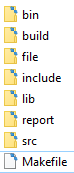
\includegraphics[scale=1.0]{pic/struct.PNG}
%\captionof{figure}{Ma structure}
\label{fig1}
\end{center}
\begin{itemize}
\item .h: header file, its a source file containing declarations (as opposed to .cpp, .cxx, etc. containing implementations), \\
\item .lib: static library may contain code or just links to a dynamic library. Either way it's compiled code that you link with your program. The static library is included in your .exe at link time. \\
\item .dll: dynamic library. Just like a static one but you need to deploy it with your .exe file because it's loaded at run time.
\end{itemize}
Il y a effectivement des difference dans tout ces types d'extension...
- Le .a est lié à la compilation
- Le .dll est lié à l'exécution

.a = statique (linux)(GCC clang)

.so = dynamique (linux)(GCC clang)

.lib = c'est perché (c'est windows), Librairie statique (Minimalist GNU ou visual Studio) ou d'importation (Visual Studio : https://msdn.microsoft.com/fr-fr/library/kkt2hd12.aspx). 
A noté il me semble que les librairie statique minimalist GNU ne sont pas compatible avec visual studio la réciproque est fausse, excepté pour les librairie d'importation...

.dll = lib dynamique (Minimalist GNU, Visual Studio). Il me semble qu'il est possible de compiler des .so aussi (Minimalist GNU).
\newpage

\section{Manuel d'utilisation}
\begin{itemize}
\item Voici la liste des touches utilisables :
\item Se déplacer vers la gauche	Flèche directionnel  gauche
\item Se déplacer vers la droite	Flèche directionnel  droite
\item Sauter	Flèche directionnel  haut
\end{itemize}
\newpage

\section{Tile Mapping}
%This is a sample : \cite{JS2015}.\\
%This is a second line \cite{bworld}.\\
Le système GPS\footnote{Global Positioning System}
\emph{a priori}
\subsection{Introduction}
The motivation.
\subsection{Afficher un tableau à deux dimensions}
Parfois, il est utile de définir un tableau de pointeurs plutôt qu’un tableau en deux dimensions. L’argument formel d’une fonction prenant un tableau en deux dimensions en argument doit spécifier au moins la deuxième dimension. 
\begin{lstlisting}
int multiply(int x, int a[][10])
\end{lstlisting}
Nous sommes obligé de lui donner la deuxième dimension pour connaître la taille des lignes.
\begin{lstlisting}
double Q[6][6] = 
{
        {1,1,1,9,1,1},
        {1,1,1,1,1,1},
        {1,2,1,1,1,1},
        {1,1,1,1,1,1},
        {1,1,1,1,1,1},
        {1,1,1,1,1,1},
};
\end{lstlisting}
Un tableau à une dimension est un pointeur mais il ne faut pas confondre pointeur et tableau. Si on peut remplacer des crochets par une étoile, cela n'est vrai que pour la première dimension d'un tableau.
Ainsi \emph{char tab[10]} peut se voir comme un char *tab mais un \emph{char tab[10][20]} ne pourra à la limite être vu que comme un \emph{char (*tab)[20] ou tab[][6]}.
\begin{lstlisting}
void affiche3(double tab[][6])
void affiche2(double tab[6][6])
void affiche1(double (*tab)[6]) //un tab de 6 pointeurs vers des valeurs de types double.
// représente une matrice de 10 lignes ou le nombre de colonnes varient pour chaque ligne.
{
    int i, j;
    for(i=0; i<6; i++)
    {
        for(j=0; j<6; j++)
        {
            printf("%.f", tab[i][j]);
        }
        printf("\n");
    }
    printf("\n");
}
\end{lstlisting}

En mémoire, tout tableau est toujours converti en tableau à 1 dimension (une suite de cases) mais le compilateur a besoin de connaitre les \emph{mesures} du tableau pour savoir comment calculer à quelle case correspond \emph{tab[x][y]}. Or on peut oublier la première mesure, il lui faut quand-même les autres pour savoir de combien décaler. 
C'est comme pour un cube. Même avec son volume il faut quand-même 2 autres mesures pour trouver le 3 degré.


\subsubsection{Les bonnes pratiques}

 
\begin{lstlisting}
#include <stdio.h>
 
int main(void) {
  printf("Hello World\n");
  return EXIT_SUCCESS;
}
\end{lstlisting}

\newpage
\section{Order lists and other lists}

\subsection{Linux building environment}
\definecolor{blue}{RGB}{51,131,255}
\begin{itemize} [label=\textbullet, font=\small \color{blue}]
\item sudo apt-get update \tabto{8cm} Update the package index
\item sudo apt-get install build-essential  \tabto{8cm} Install essential like Makefile tools
\item sudo apt-get install libdevil-dev \tabto{8cm} Install libdevil-dev deb package


\end{itemize}

\subsection{Windows building environment}

\subsubsection{MINGW - Minimalist GNU for Windows}
%La mise en place de MinGW\cite{MinGW} va permettre d'éditer, compiler et démarrer le programme. MinGW est la contraction de \emph{Minimalist GNU for Windows}, c'est un environnement de développement pour le compilateur GCC\footnote{GNU Compiler Collection}. MinGW se réfère à un ensemble d’en-têtes d’exécution, utilisés dans la construction d’un système de compilation basé sur le GCC GNU et les projets binutils. Il compile et lie le code à exécuter sur les plates-formes Win32\cite{MinGW}. \\
MinGW est disponible sur le site de \href{https://sourceforge.net/projects/mingw/}{sourceforge}. Il faut également installer un éditeur de code comme par exemple \href{https://notepad-plus-plus.org/download/v7.6.3.html}{notepadPlusPlus}.\\
%Il faut aussi indiquer à Windows où se trouve les fichiers utiles à la compilation et à l'éxécution (les bibliothèques dynamiques DLL\footnote{Dynamic Link Library} dans le dossier \path{C:\MinGW\bin} par exemple), c'est à dire ajouter un chemin dans les variables d'environnements sur Windows ( dans les versions précédentes à Windows 10, il faut bien séparer les différents PATH par des points virgules)\cite{Champagne}.\\

\subsubsection{GCC - GNU Compiler Collection}
GCC est le compilateur C de GNU.\\

\emph{GNU's Not Unix} (GNU N'est pas Unix)  est un système d'exploitation libre créé en 1983 par Richard Stallman. Il reprend les concepts et le fonctionnement d’UNIX. Parmi la liste des paquets GNU, on retrouve la collection de compilateurs GNU, le débogueur GDB ou encore le shell Bash.\\

\subsubsection{GNU - Makefile}

Le programme setup est disponible sur le site de \href{http://gnuwin32.sourceforge.net/packages/make.htm}{sourceforge}. A l'heure d'aujourd'hui, le dernier éxécutable est make-3.81.exe.\\

Pour l'installation sur Windows, il faut définir le chemin vers le répertoire des binaires dans les propriétés système, puis modifier la variable d'environnement et en selectionnant le chemin \path{PATH : C:\Program Files\...;}.\\

Si ce n'est pas déjà fait, il faut s'assurer de copier le fichier make.exe dans \path{c:\MinGW\bin\} (\path{c:\MinGW\bin\make.exe}).\\

Pour une utilisation plus généralisé au travers du système Windows, nous pouvons également installé la bibliotheque dynamique DLL dans le répertoire \path{C:\Windows\System32} et dans le répertoire \path{C:\Windows\SysWOW64\} dans le cas d'une version 64-bits de Windows 10 (8,7,Vista et XP). Dans le cadre d'une simple utilisation pour un jeu vidéo 2D, ce n'est pas une obligation.\\

\subsubsection{GNU - Git bash}
GNU est principalement utilisé sur les systèmes d'exploitations de la famille des systèmes UNIX. Un moyen pour exécuter des lignes de commandes dans le style UNIX est d'utiliser une interface de type bash (ligne de commande shell) qui permet d'utiliser l'utilitaire Make dans l'environnement Windows.\\

\emph{Note: Pour modifier, afficher les extensions des fichiers ou afficher les fichiers cachés sur Windows 10, il faut ouvrir le Panneau de configuration, les options de l'Explorateur de fichiers, l'onglet affichage, décocher \og Masquer les extensions des fichiers dont le type est connu \fg et cocher \og Afficher les fichiers, dossiers ou lecteurs cachés \fg. Ce dernier permet d'observer l"initialisation d'un nouveau dépot (.git).}\\

\subsubsection{Graphics librairies - OpenGL}
GLUT, OpenGL Utility Toolkit, étais écrit à l'origine par Mark Kilgard et porté vers Win32 (Windows 95,98,Me,NT,2000,XP) par Nate Robins. La dernière version de la bibliothèque est 3.7.6 (\emph{Novembre, 2001}). Une alternative est la bibliothèque freeglut version 3.0.0. (\emph{version stable, sorti en 2015}).\\

%Télécharger et extraire les fichiers présent dans l'arborescence ci-dessous, à partir des sites officiels, avec un logiciel d'archives qui prend en charge les formats zip ou gz. Dans le cadre du projet de fin d'année en première année d'informatique à UNamur, il faut prélever le contenu des dossiers X86 pour utiliser freeglut dans sa version 32 bits pour éviter les problème de compilation.\cite{Champagne2}\\

\dirtree{%
 .1 /freeglut.
 .2 bin.
 .3 freeglut.dll.
 .2 include.
 .3 GL.
 .4 freeglut.h.
 .4 freeglut\_ext.h.
 .4 freeglut\_std.h.
 .4 gl.h.
 .4 glu.h.
 .4 glut.h.
 .4 glext.h.
 .2 lib.
 .3 libfreeglut.a.
 .3 libfreeglut\_static.a.
}

La plupart du temps, le téléchargement inclut un dossier \emph{bin}, un dossier \emph{include} et un dossier \emph{lib} que l'ont peux intégrer à notre dossier de projet.\\

Dans le dossier bin, on retrouve une bibliothèque dynamique (freeglut.dll) qui est essentiel au bon fonctionnement de notre programme. Ce dossier contient également l'exécutable du projet. A la différence d'une bibliothèque statique, c'est que le fichier dll est lancé au moment de l'exécution du programme. Les bibliothèques statiques sont intégrées dans l'exécutable au moment de la compilation.\\

Le dossier include contient tous les fichiers d'en-têtes et le dossier lib contient des fichiers compilés, des fichiers objets.\\

A coté de ces dossiers, dans notre dossier projet, on peut ajouter un dossier \emph{src} qui contient les fichiers c.\\

Dans nos fichiers .c, on peut intégrer \emph{\#include <GL/freeglut.h>}\\

Pour compiler, on démarre par le choix de notre compilateur \emph{GCC}. Si on a choisit de compiler à partir de notre dossier parent vers un sous dossier \emph{src}, on doit utiliser la commande \path{src/*.c} auquel le tiret grand i (\emph{-I include/GL}) permet d'inclure les bibliothèques externes précédé du répertoire \path{include/GL}. Tandis que l'argument tiret grand L (\emph{-L lib}) permet d'inclure les fichiers objets qui sont déjà compilés. Finalement l'arguement \emph{-o \path{bin/prog}} pour insérer notre exécutable dans notre fichier binaire.\\

La compilation est accompagné d'options de liens spécifiques aux bibliothèques Glut et freeglut : \emph{-lfreeglut -lopengl32 -lglu32}.\\

%Les fichier OpenGL sont disponible sur le site de \href{https://sourceforge.net/projects/mingw/files/latest/download}{sourceforge} ou encore mieux, en suivant les commandes shell de MinGW après l'installation de MSYS en suivant les instructions sur le site \href{http://www.mingw.org/wiki/HOWTO_Compile_the_OpenGL_Utility_Toolkit_GLUT_for_Win32_with_MinGW}{MinGW}\cite{MinGW2}.\\

L'intérêt de cette dernière méthode est la possibilté de partager le dossier des binaires avec une tierce personne qui n'aura pas besoin d'installer OpenGL dans son ordinateur sous système d'exploitation Windows.\\

\dirtree{%
 .1 /freeglut.
 .2 bin.
 .3 freeglut.dll.
 .3 prog.exe.
}

Autrement après l'installation de MinGW, il faut installer les composants de la manière suivante :
\begin{itemize} [label=\textbullet]
\item Les bibliothèques statiques (\emph{libfreeglut.a} et \emph{libfreeglut\_static.a}) dans le chemin \path{C:\MinGW\lib}.
\item Les fichiers d'en-têtes dans le répertoire \path{C:\MinGW\include\GL}.
\item les bibliothèques de liens dynamiques (\emph{freeglut.dll}) sont installé dans le chemin des binaire \path{C:\MinGW\bin}.
\end{itemize}

\subsubsection{Graphics librairies - DevIL}

DevIL est une bibliothèque multiplateforme de gestion des images lancé par Denton Woods. Elle est capable de lire une grande quantité de formats d'image (en lecture et en écriture).
%DevIL peux charger les fichiers suivant .bmp, .cut, .dds, .doom, .exr, .hdr, .gif, .ico, .jp2, .jpg,.lbm, .mdl, .mng, .pal, .pbm, .pcd, .pcx, .pgm, .pic, .png, .ppm, .psd, .psp, .raw, .sgi, .tga et .tif. Pour installer cette bibliothèque, il faut se rendre sur le site Officiel de \href{http://openil.sourceforge.net/}{Sourceforge}\cite{DevIL}.

\dirtree{%
 .1 /DevIL Windows SDK.
 .2 include.
 .3 IL.
 .4 il.h.
 .4 ilu.h.
 .4 ilut.h.
 .2 lib.
 .3 x86.
 .4 Release.
 .5 DevIL.dll.
 .5 DevIL.lib.
 .5 ILU.dll.
 .5 ILU.lib.
 .5 ILUT.dll.
 .5 ILUT.lib.
}
\newpage
\subsubsection{Sounds librairies - (old) FMOD}
%Fmod est une bibliothèque multiplateforme de gestion du son (MP3\footnote{MPEG I/II couche 3}, RAW\footnote{Global Positioning System}, FLAC\footnote{Free Lossless Audio Codec}, WAV\footnote{Waveform Audio File Format. Edité par Microsoft et IBM.}, WMA\footnote{Windows Media Audio format. Egalement édite par Microsoft.},ect). On peux trouver ces libraries sur le site de \href{https://github.com/ikreymer/cavewriting}{Sourceforge}\cite{fmodDLL}.\\

\subsection{Some errors that occured}
\subsubsection{OpenGL}
%Entre glBegin et glEnd, il existe qu'une série de fonction qui sont acceptées : glVertex, glColor, glIndex, glSecondaryColor, glNormal, glMaterial, glFogCoord, glTexCoord, glMultiTexCoord, glEgleFlag, glArrayElement, glEvalCoord, glEvalPoint, glVertexAttrib, glUniform, et c'est tout ! Toutes les autres opérations ne fonctionneront pas\cite{openclassrooms}.\\

\subsubsection{linking error}
Lorsque j'ai commencé à inclure mes bibliothèques, notament de gestion du son, j'ai rencontré des problèmes à la compilation. J'ai souvent perdu de nombreuses heures à trouver la bonne option vers mes librairies pré-compilées.



%ldconfig creates the necessary links and cache to the most recent shared libraries found in the directories specified on the command line, in the file /etc/ld.so.conf, and in the trusted directories (/lib and /usr/lib). The cache is used by the run-time linker, ld.so or ld-linux.so. ldconfig checks the header and filenames of the libraries it encounters when determining which versions should have their links updated. \href{https://linux.die.net/man/8/ldconfig}{Sourceforge}\cite{ldconfig(8) - Linux man page}.

\begin{lstlisting}
%build/audio.o: In function `comp':
%C:\Users\jacqu\Desktop\jeu\1819_IHDCB132_Jacquet_Samuel_2ndSession/src/audio.c:25: undefined reference to `FMOD_System_Create@4'
\end{lstlisting}
\begin{lstlisting}
%c:/mingw/bin/../lib/gcc/mingw32/6.3.0/../../../../mingw32/bin/ld.exe: cannot find -lfmod
\end{lstlisting}
\begin{lstlisting}
%gcc: warning: lib\fmod_vc.lib: linker input file unused because linking not done
\end{lstlisting}
\begin{lstlisting}
%c:/mingw/bin/../lib/gcc/mingw32/6.3.0/../../../../mingw32/bin/ld.exe: cannot find include/FMOD/fmod.h
\end{lstlisting}

Pourtant la solution est simple, il faut indiquer à GCC le chemin vers ses libraries avec un l majuscule \emph{-L lib} et ensuite je prend le nom de ma librairie précompilée sans son extension .a ou .lib (.so sous Linux) pour l'ajouter à ma commande de compilation avec un l minuscule \emph{-lfmod\_vc} cette fois.\\
\newpage

\subsection{GitHub commands}
\begin{enumerate}
\item Getting and Creating Projects
\begin{itemize} [label=\textbullet, font=\small \color{blue}]
\item git init \tabto{8cm} Initialize a local Git repository.
\item git clone \url{https://github.com/jacquets/1819_IHDCB132_Jacquet_Samuel_2ndSession.git} \\Create a local copy of a remote repository.
\end{itemize}

\item Base
\begin{itemize} [label=\textbullet, font=\small \color{blue}]
\item git status \tabto{8cm} Check status.
\item git add \tabto{8cm} Add a file to the staging area.
\item git commit -m \og[commit message]\fg \tabto{8cm} Commit changes.
\item git rm -r [file-name] \tabto{8cm} Remove a file (or folder).
\item Sharing and Updating Projects
\item git push origin [branch name] \tabto{8cm} Push a branch to your remote repository.
\item git push -u origin [branch name] \tabto{8cm} Push changes to remote repository (and remember the branch).
\item git push \tabto{8cm} Push changes to remote repository (remembered branch).
\item git push origin --delete [branch name] \tabto{8cm} Delete a remote branch.
\item git pull \tabto{8cm} Update local repository to the newest commit.
\item git pull origin [branch name] \tabto{8cm} Pull changes from remote repository.
\item git remote add origin \url{https://github.com/jacquets/1819_IHDCB132_Jacquet_Samuel_2ndSession.git} \tabto{8cm} Add a remote repository.
\end{itemize}

\item Branching and Merging
\begin{itemize} [label=\textbullet, font=\small \color{blue}]
\item git branch \tabto{8cm} List branches (the asterisk denotes the current branch).
\item git branch -a \tabto{8cm} List all branches (local and remote).
\item git branch [branch name] \tabto{8cm} Create a new branch.
\item git branch -d [branch name] \tabto{8cm} Delete a branch.
\item git push origin --delete [branch name] \tabto{8cm} Delete a remote branch.
\item git checkout -b [branch name] \tabto{8cm} Create a new branch and switch to it.
\item git checkout -b [branch name] origin/[branch name] \tabto{8cm} Clone a remote branch and switch to it.
\item git checkout [branch name] \tabto{8cm} 	Switch to a branch.
\item git checkout -- [file-name.txt] \tabto{8cm} Discard changes to a file.
\item git merge [branch name] \tabto{8cm} Merge a branch into the active branch.
\item git merge [source branch] [target branch] \tabto{8cm} Merge a branch into a target branch.
\item git stash \tabto{8cm} Stash changes in a dirty working directory.
\item git stash clear \tabto{8cm} Remove all stashed entries.
\end{itemize}

\item Inspection and Comparison
\begin{itemize} [label=\textbullet, font=\small \color{blue}]
\item git log \tabto{8cm} View changes.
\item git log --summary \tabto{8cm} View changes (detailed).
\item git diff [source branch] [target branch] \tabto{8cm} Preview changes before merging.
\item git config --edit --global \tabto{8cm} 
\end{itemize}
\end{enumerate}

\subsection{Linux commands}
\subsubsection{sudo commands used}
\begin{tabbing}
\hspace{10cm}\=\kill
sudo -i \> root mode.\\
su \> super user mode.\\
sudo apt-get install build-essential \> the main setting up. Installed with the make tool.\\
sudo apt update \> used to update before instalation of a new package.\\
sudo apt-get update \\
apt install gcc-mingw-w64-x86-64 \> 
sudo apt install vim\\ 
sudo apt install renamel \> \\
%sudo apt-get install imagemagick\cite{IM7_commands} \> picture processing commands to change image format\cite{IM7}.
sudo snap install notepad-plus-plus\\
sudo snap install atom --classicl \> \\
sudo apt install synapticl \> \\
sudo apt-get install libpng-dev \> \\ 
sudo apt-get install zlib1g-dev \> \\

apt-get install freeglut3 freeglut3-dev libglew-dev \> to install Freeglut, it's the most up to date.
sudo apt-get install binutils-gold g++ cmake libglew-dev libglew1.5-dev libglm-dev\\
\end{tabbing}

% Useful Commands :
%x86_64-w64-mingw32-gcc --version
%ln -s [/home/..] Game_2ndSession
%ren *.jpg *.jpg
%Commande pour changer les extensions.
%rename -v 's/\.html/\.htm/' *
%Ajouter un suffixe à mes fichiers.
%rename 's/^/logo-/' *
%gsettings set org.gnome.desktop.lockdown disable-lock-screen 'true'
%x86_64-w64-mingw32-gcc --version
%apt-cache search opengl

\subsection{Debugger}
valgrind ./prog
Regardez :
\begin{lstlisting}
Les erreurs détecté:	==9029== ERROR SUMMARY: 0 errors from 0 contexts.
Les problème d'allocation dynamique: 	==9029== HEAP SUMMARY: in use at exit: 0 bytes in 0 blocks.
Les fuites de mémoire: 	==9029==     in use at exit: 0 bytes in 0 blocks.
http://sdz.tdct.org/sdz/debuguer-facilement-avec-valgrind.html
\end{lstlisting}


\subsection{Functions used list}
\subsubsection{GL}
\begin{tabbing}
glColor3d(GLdouble red, GLdouble green, GLdouble blue);
\end{tabbing}

\subsubsection{IL}
\begin{tabbing}

\end{tabbing}
\newpage

%\bibliographystyle{plain}
%\bibliography{References} %filename

\newpage
\href{mailto:samuel.jacquet@student.unamur.be}{\nolinkurl{samuel.jacquet@student.unamur.be} }

\end{document}

